% Diagrama de fluxo de dados ilustrativo do estudo (segunda etapa da monografia).
% Elementos ilustrativos esquemáticos desenhados pelos autores; sem fotografias.
% Compilar com: pdflatex dataflow-tcc2.tex
\documentclass[tikz,border=8pt]{standalone}
\usepackage[T1]{fontenc}
\usepackage[utf8]{inputenc}
\usepackage{lmodern}
\usepackage{graphicx}
\graphicspath{{img/}}
\usetikzlibrary{arrows.meta,positioning,calc,shapes.geometric}

\definecolor{escuro}{HTML}{26365B}
\definecolor{azul}{HTML}{2453A6}
\definecolor{medio}{HTML}{7FC2E3}
\definecolor{claro}{HTML}{E3F1F9}
\definecolor{cinza}{HTML}{6B7487}
\definecolor{cinzaclaro}{HTML}{EEF0F4}
\definecolor{derm}{HTML}{B4532A}
\definecolor{dermclaro}{HTML}{FBEAE2}

\begin{document}
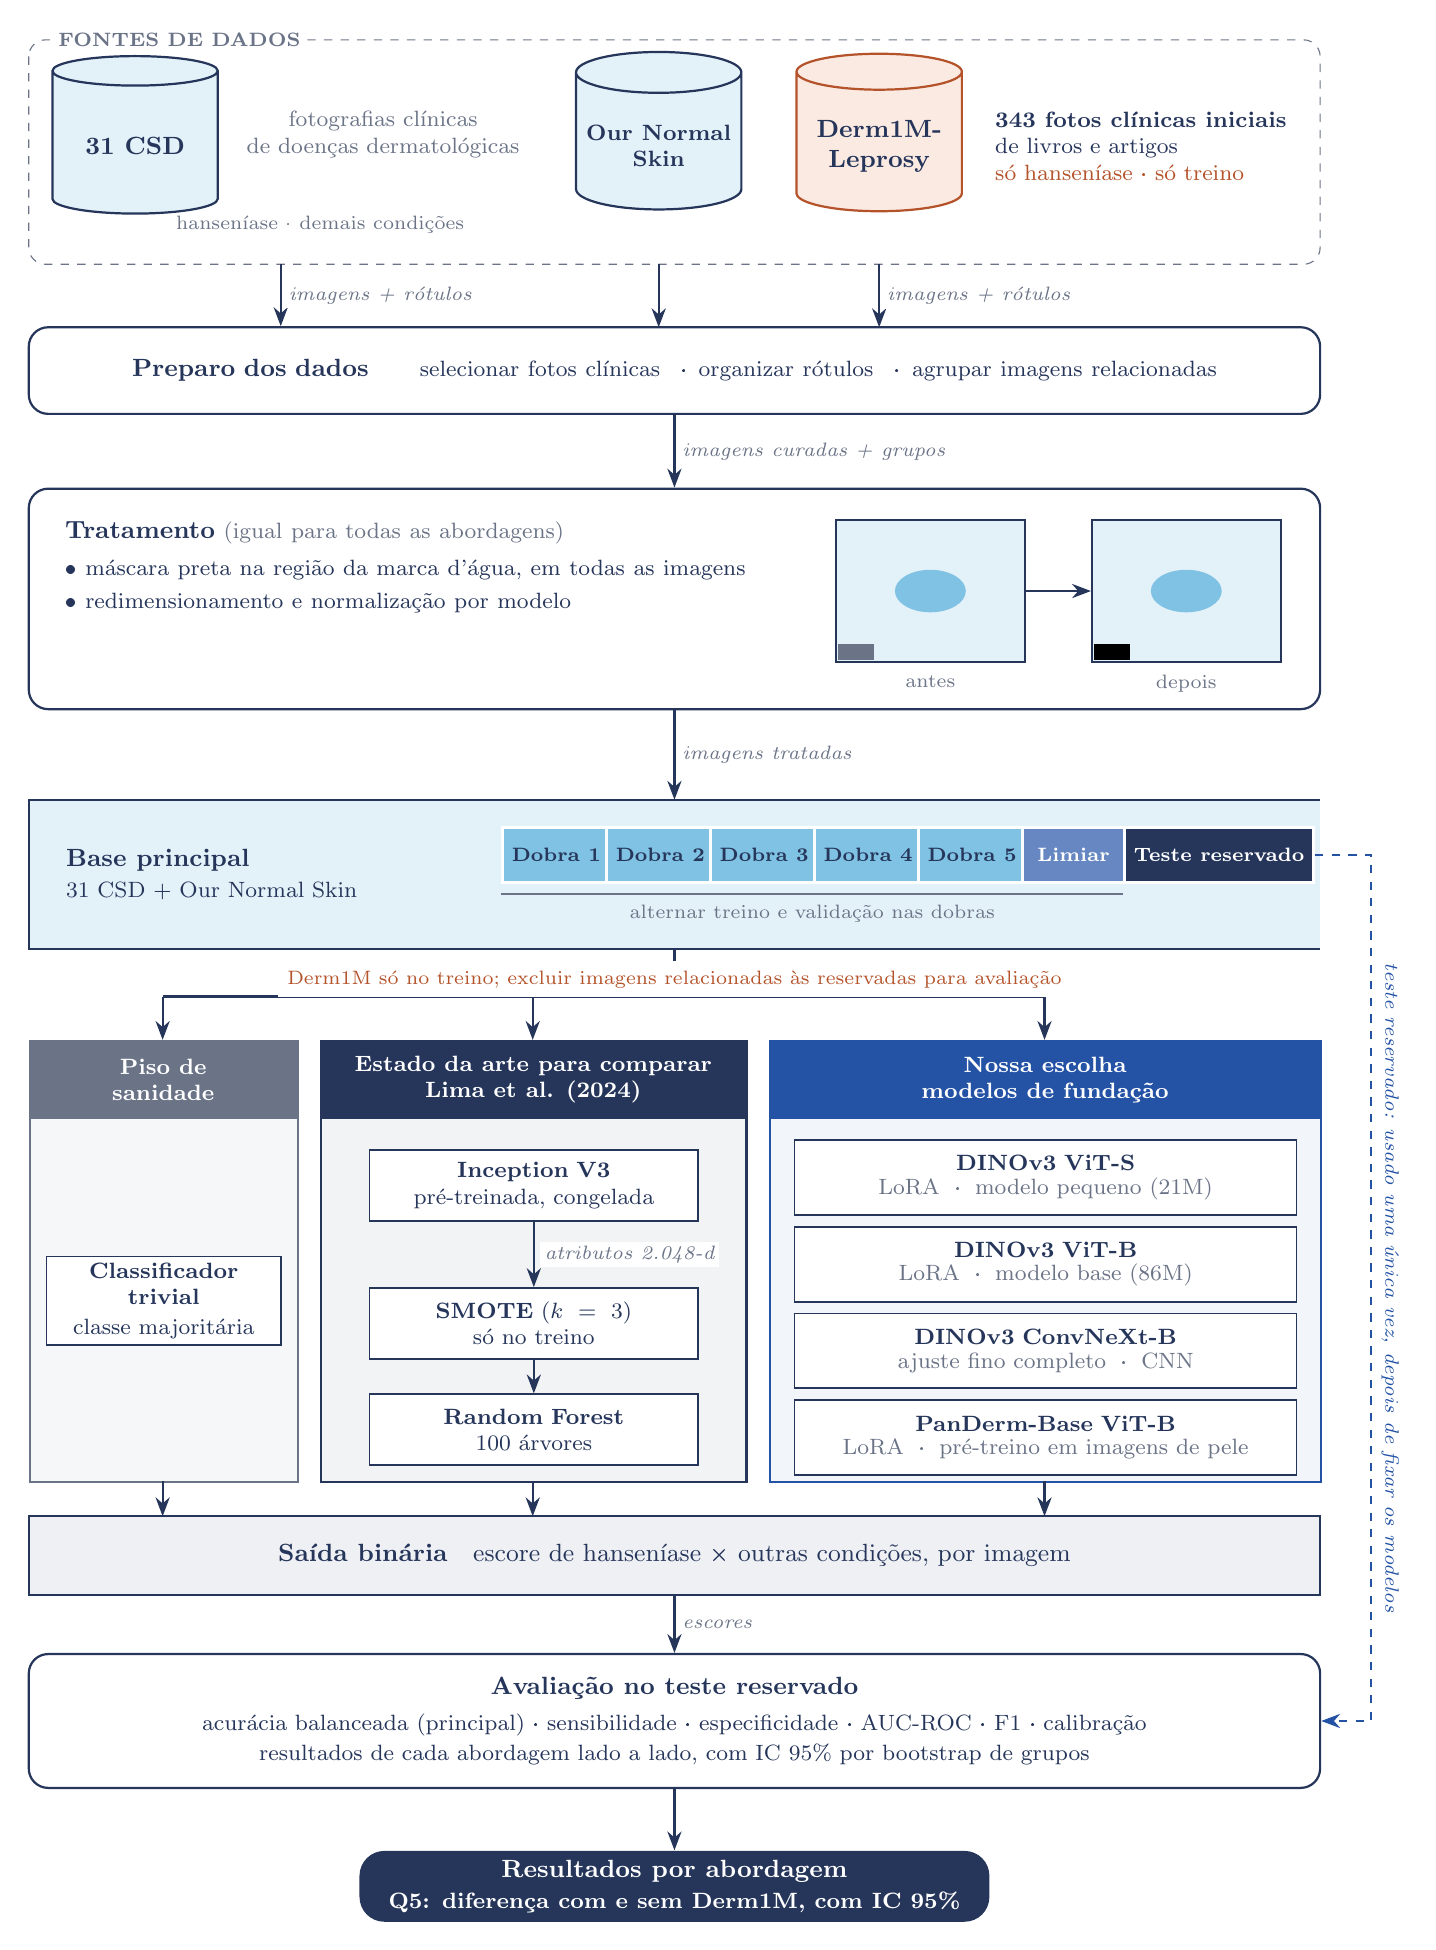
\begin{tikzpicture}[
	font=\small, text=escuro,
	>={Stealth[length=2.4mm]},
	fluxo/.style={->, thick, escuro},
	rot/.style={font=\scriptsize\itshape, text=cinza, fill=white, inner sep=1.5pt},
	base/.style={cylinder, shape border rotate=90, aspect=0.25, draw=escuro, thick,
		minimum width=21mm, minimum height=20mm, align=center, font=\small\bfseries},
	proc/.style={rectangle, rounded corners=7pt, draw=escuro, thick, fill=white},
	caixa/.style={rectangle, draw=escuro, semithick, fill=white, align=center,
		minimum height=9mm, inner sep=2.5pt, font=\footnotesize},
	cab/.style={rectangle, minimum height=10mm, align=center, font=\footnotesize\bfseries, text=white, inner sep=2pt},
	grupo/.style={rectangle, draw=#1, thick, fill=#1!6},
	foto/.style={inner sep=0pt, draw=escuro, semithick},
]
% Largura útil: x de 0.3 a 16.7 (164 mm)

% =============== 1. FONTES DE DADOS ===============
\draw[cinza, dashed, rounded corners=6pt] (0.3,-0.1) rectangle (16.7,-2.95);
\node[font=\scriptsize\bfseries, text=cinza, fill=white, inner sep=2pt, anchor=west] at (0.6,-0.1) {FONTES DE DADOS};

\node[base, fill=claro] (csd) at (1.65,-1.45) {31 CSD};
\node[font=\footnotesize, align=center, text=cinza] at (4.8,-1.3) {fotografias clínicas\\de doenças dermatológicas};

\node[base, fill=claro, font=\footnotesize\bfseries] (normal) at (8.3,-1.45) {Our Normal\\Skin};
\node[font=\scriptsize, text=cinza, align=center] at (4.0,-2.45)
	{hanseníase · demais condições};

\node[base, fill=dermclaro, draw=derm] (dm) at (11.1,-1.45) {Derm1M-\\Leprosy};
\node[align=left, font=\footnotesize, anchor=west] at (12.45,-1.45)
	{\textbf{343 fotos clínicas iniciais}\\de livros e artigos\\{\color{derm}só hanseníase · só treino}};

% =============== 2. CURADORIA ===============
\node[proc, minimum width=164mm, minimum height=11mm, text width=158mm, align=center] (cur) at (8.5,-4.3)
	{\textbf{Preparo dos dados}\qquad {\footnotesize selecionar fotos clínicas
	 \enspace·\enspace organizar rótulos
	 \enspace·\enspace agrupar imagens relacionadas}};
\coordinate (xcsd) at (3.5,0);
\draw[fluxo] (3.5,-2.95) -- node[rot, right=1pt] {imagens + rótulos} (xcsd |- cur.north);
\draw[fluxo] (8.3,-2.95) -- (8.3,-3.75);
\draw[fluxo] (11.1,-2.95) -- node[rot, right=1pt] {imagens + rótulos} (11.1,-3.75);

% =============== 3. TRATAMENTO ===============
\node[proc, minimum width=164mm, minimum height=28mm] (tra) at (8.5,-7.2) {};
\node[anchor=north west, align=left, text width=92mm] at ($(tra.north west)+(0.35,-0.3)$)
	{\textbf{Tratamento} \textcolor{cinza}{\footnotesize(igual para todas as abordagens)}\\[4pt]
	 \footnotesize
	 \textbullet\ máscara preta na região da marca d'água, em todas as imagens\\[1pt]
	 \textbullet\ redimensionamento e normalização por modelo};
\node[foto, minimum width=24mm, minimum height=18mm, fill=claro] (antes) at (11.75,-7.1) {};
\fill[medio] (11.75,-7.1) ellipse (0.45 and 0.27);
\fill[cinza] ($(antes.south west)+(0.04,0.04)$) rectangle ++(0.45,0.20);
\node[foto, minimum width=24mm, minimum height=18mm, fill=claro] (depois) at (15.0,-7.1) {};
\fill[medio] (15.0,-7.1) ellipse (0.45 and 0.27);
\fill[black] ($(depois.south west)+(0.04,0.04)$) rectangle ++(0.45,0.20);
\draw[fluxo] (antes.east) -- (depois.west);
\node[font=\scriptsize, text=cinza, below=1pt of antes] {antes};
\node[font=\scriptsize, text=cinza, below=1pt of depois] {depois};
\draw[fluxo] (cur.south) -- node[rot, right=1pt] {imagens curadas + grupos} (cur.south |- tra.north);

% =============== 4. PARTIÇÕES (depósito de dados) ===============
\fill[claro] (0.3,-9.75) rectangle (16.7,-11.65);
\draw[escuro, thick] (16.7,-9.75) -- (0.3,-9.75) -- (0.3,-11.65) -- (16.7,-11.65);
\node[anchor=west, align=left] at (0.65,-10.7)
	{\textbf{Base principal}\\{\footnotesize 31 CSD + Our Normal Skin}};
\foreach \i/\x in {1/6.3,2/7.62,3/8.94,4/10.26,5/11.58}{
	\node[rectangle, fill=medio, draw=white, line width=1pt, minimum width=13.2mm, minimum height=7mm,
		font=\scriptsize\bfseries, anchor=west] at (\x,-10.45) {Dobra \i};
}
\node[rectangle, fill=azul!70, draw=white, line width=1pt, minimum width=13mm, minimum height=7mm,
	font=\scriptsize\bfseries, text=white, anchor=west] at (12.9,-10.45) {Limiar};
\node[rectangle, fill=escuro, draw=white, line width=1pt, minimum width=24mm, minimum height=7mm,
	font=\scriptsize\bfseries, text=white, anchor=west, align=center] (teste) at (14.2,-10.45) {Teste reservado};
\draw[cinza, semithick] (6.3,-10.95) -- (14.2,-10.95);
\node[font=\scriptsize, text=cinza] at (10.25,-11.2) {alternar treino e validação nas dobras};
\draw[fluxo] (tra.south) -- node[rot, right=1pt] {imagens tratadas} (8.5,-9.75);

% =============== 5. ABORDAGENS ===============
% distribuição das dobras para os três grupos
\draw[thick, escuro] (8.5,-11.65) -- (8.5,-12.25);
\draw[thick, escuro] (2.0,-12.25) -- (13.2,-12.25);
\foreach \x in {2.0,6.7,13.2}{ \draw[fluxo] (\x,-12.25) -- (\x,-12.8); }
\node[font=\scriptsize, text=derm, align=center, fill=white] at (8.5,-12.03)
	{Derm1M só no treino; excluir imagens relacionadas às reservadas para avaliação};

% Grupo 1: piso
\node[grupo=cinza, minimum width=34mm, minimum height=56mm, anchor=north west] (g1) at (0.3,-12.8) {};
\node[cab, fill=cinza, minimum width=34mm, anchor=north west] at (g1.north west) {Piso de\\sanidade};
\node[caixa, text width=28mm] (triv) at ($(g1.center)+(0,-0.5)$) {\textbf{Classificador}\\\textbf{trivial}\\[1pt]classe majoritária};

% Grupo 2: Lima
\node[grupo=escuro, minimum width=54mm, minimum height=56mm, anchor=north west] (g2) at (4.0,-12.8) {};
\node[cab, fill=escuro, minimum width=54mm, anchor=north west] at (g2.north west) {Estado da arte para comparar\\Lima et al. (2024)};
\node[caixa, text width=40mm] (inc) at ($(g2.north)+(0,-1.85)$) {\textbf{Inception V3}\\pré-treinada, congelada};
\node[caixa, text width=40mm] (smo) at ($(g2.north)+(0,-3.6)$) {\textbf{SMOTE} ($k = 3$)\\só no treino};
\node[caixa, text width=40mm] (rf)  at ($(g2.north)+(0,-4.95)$) {\textbf{Random Forest}\\100 árvores};
\draw[fluxo] (inc) -- node[rot, right=2pt] {atributos 2.048-d} (smo);
\draw[fluxo] (smo) -- (rf);

% Grupo 3: nossa escolha
\node[grupo=azul, minimum width=70mm, minimum height=56mm, anchor=north west] (g3) at (9.7,-12.8) {};
\node[cab, fill=azul, minimum width=70mm, anchor=north west] at (g3.north west) {Nossa escolha\\modelos de fundação};
\foreach \n/\t/\a/\dy in {
	vis/{DINOv3 ViT-S}/{LoRA \;·\; modelo pequeno (21M)}/1.75,
	vib/{DINOv3 ViT-B}/{LoRA \;·\; modelo base (86M)}/2.85,
	cnx/{DINOv3 ConvNeXt-B}/{ajuste fino completo \;·\; CNN}/3.95,
	pan/{PanDerm-Base ViT-B}/{LoRA \;·\; pré-treino em imagens de pele}/5.05}{
	\node[caixa, text width=62mm, minimum height=9.5mm] (\n) at ($(g3.north)+(0,-\dy)$)
		{\textbf{\t}\\[-1pt]\textcolor{cinza}{\a}};
}

% =============== 6. SAÍDA BINÁRIA ===============
\foreach \x in {2.0,6.7,13.2}{ \draw[fluxo] (\x,-18.4) -- (\x,-18.85); }
\node[rectangle, fill=cinzaclaro, draw=escuro, thick, minimum width=164mm, minimum height=10mm,
	align=center] (sai) at (8.5,-19.35)
	{\textbf{Saída binária}\quad escore de hanseníase × outras condições, por imagem};

% =============== 7. AVALIAÇÃO ===============
\node[proc, minimum width=164mm, minimum height=17mm, align=center] (ava) at (8.5,-21.45)
	{\textbf{Avaliação no teste reservado}\\[2pt]
	 \footnotesize acurácia balanceada (principal) · sensibilidade · especificidade · AUC-ROC · F1 · calibração\\
	 \footnotesize resultados de cada abordagem lado a lado, com IC 95\% por bootstrap de grupos};
\draw[fluxo] (sai.south) -- node[rot, right=1pt] {escores} (sai.south |- ava.north);

% teste reservado: segue por fora até a avaliação e é usado uma única vez
\draw[fluxo, dashed, azul] (teste.east) -- (17.35,-10.45) -- node[pos=0.5, sloped, above, font=\scriptsize\itshape, text=azul]
	{teste reservado: usado uma única vez, depois de fixar os modelos} (17.35,-21.45) -- (ava.east);

% =============== 8. RESULTADO ===============
\node[rectangle, rounded corners=9pt, fill=escuro, text=white, minimum width=80mm, minimum height=9mm,
	font=\small\bfseries, align=center] (res) at (8.5,-23.55)
	{Resultados por abordagem\\{\footnotesize Q5: diferença com e sem Derm1M, com IC 95\%}};
\draw[fluxo] (ava.south) -- (res.north);

\end{tikzpicture}
\end{document}
